\documentclass[aspectratio=169]{beamer}

%\usepackage[table]{xcolor}
\mode<presentation> {
  \usetheme{Boadilla}
%  \usetheme{Pittsburgh}
%\usefonttheme[2]{sans}
\renewcommand{\familydefault}{cmss}
%\usepackage{lmodern}
%\usepackage[T1]{fontenc}
%\usepackage{palatino}
%\usepackage{cmbright}

\useinnertheme{rectangles}
}
%\usepackage{normalem}{ulem}
%\usepackage{colortbl, textcomp}
\setbeamercolor{normal text}{fg = black}
\setbeamercolor{structure}{fg = blue}
\definecolor{trial}{cmyk}{1,0,0, 0}
\definecolor{trial2}{cmyk}{0.00,0,1, 0}
\definecolor{darkgreen}{rgb}{0,.4, 0.1}
\usepackage{array}
\beamertemplatesolidbackgroundcolor{white}  \setbeamercolor{alerted
text}{fg=red}

\setbeamertemplate{caption}[numbered]\newcounter{mylastframe}

\usepackage{color}
\usepackage{tikz}
\usepackage{hyperref}
\usetikzlibrary{arrows}
\usepackage{colortbl}
%\usepackage[usenames, dvipsnames]{color}
%\setbeamertemplate{caption}[numbered]\newcounter{mylastframe}c
%\newcolumntype{Y}{\columncolor[cmyk]{0, 0, 1, 0}\raggedright}
%\newcolumntype{C}{\columncolor[cmyk]{1, 0, 0, 0}\raggedright}
%\newcolumntype{G}{\columncolor[rgb]{0, 1, 0}\raggedright}
%\newcolumntype{R}{\columncolor[rgb]{1, 0, 0}\raggedright}
\setbeamercolor{normal text}{fg = black}
\setbeamercolor{structure}{fg = blue}
\definecolor{trial}{cmyk}{1,0,0, 0}
\definecolor{trial2}{cmyk}{0.00,0,1, 0}
\definecolor{darkgreen}{rgb}{0,.4, 0.1}
\definecolor{mygray}{gray}{0.8}
\definecolor{myblack}{rgb}{0, 0, 0}

%\begin{beamerboxesrounded}[upper=uppercol,lower=lowercol,shadow=true]{Block}
%$A = B$.
%\end{beamerboxesrounded}}
\renewcommand{\familydefault}{cmss}
%\usepackage[all]{xy}

\usepackage{tikz}
\usepackage{lipsum}

 \newenvironment{changemargin}[3]{%
 \begin{list}{}{%
 \setlength{\topsep}{0pt}%
 \setlength{\leftmargin}{#1}%
 \setlength{\rightmargin}{#2}%
 \setlength{\topmargin}{#3}%
 \setlength{\listparindent}{\parindent}%
 \setlength{\itemindent}{\parindent}%
 \setlength{\parsep}{\parskip}%
 }%
\item[]}{\end{list}}
\usetikzlibrary{arrows}
%\usepackage{palatino}
%\usepackage{eulervm}
\usecolortheme{lily}

\newtheorem{com}{Comment}
\newtheorem{lem} {Lemma}
\newtheorem{prop}{Proposition}
\newtheorem{thm}{Theorem}
\newtheorem{defn}{Definition}
\newtheorem{cor}{Corollary}
\newtheorem{obs}{Observation}
 \numberwithin{equation}{section}
\setbeamertemplate{navigation symbols}{}


\title[PLSC 43401]{Mathematical Foundations of Political Methodology Lecture 1}

\author{Robert Gulotty}
\institute[University of Chicago]{Department of Political Science \\  University of Chicago}
\vspace{0.3in}
\date{}

\begin{document}



\begin{frame}
\titlepage
\end{frame}



\begin{frame}{Political Methodology at Chicago}

\begin{itemize}
\item This Course (PLSC 43401)
\begin{itemize}
\item Calculus/Linear Algebra, Probability/Statistics
\item Formal Track:  Game Theory I, Game Theory II, Formal Models of Domestic Politics; [New topics in Formal Models or Social Choice.]
\item Quantitative Track:  Linear Models, Political Economy II (Zelizer), [MLE or Multilevel Models etc.]
\end{itemize}
\item Computational Tools for Social Science (R. Terman) (PLSC 31101)
\begin{itemize}
\item Computational techniques, Replicable coding practices.
\item Uses: Everyday programming, writing/publishing papers. 
\end{itemize}
\end{itemize}
\end{frame}


\begin{frame}{Comments on Math and Politics}
\begin{itemize}
\item This is not what the typical political scientist signed up for.\pause
\item Do not skip steps.  If you lack high school math, get high school math, there are many resources online.\pause
\item Textbooks are your friend.  
\begin{itemize}
\item Unlike other classes, the textbook here is necessary.
\item Ideally, 20 pages $\sim$ 2 hours, but even a single page can be an hour.
\item Sometimes you need to make up new problems for yourself, test yourself as you go.
\item We will be having weekly, in class quizzes on the readings (the first is available on Canvas).
\end{itemize}
\end{itemize}


\end{frame}


\begin{frame}{A few notes on difficulty}

\begin{itemize}

\item This course is the broadest offered in the department: we cover 300+ years of mathematical insights. \pause Don't expect your understanding to be immediate.\pause
\item Mathematical training has advantages, in part because we know where students trip up.
\item ``The Owl of Minerva begins its flight at the break of dawn.'' -Hegel 


\end{itemize}

\end{frame}


\begin{frame}{Resources}

\begin{itemize}
\item Math
\begin{itemize}
\item Siegel and Moore \emph{A Mathematics Course for Political and Social Research} \href{http://people.duke.edu/~das76/Mathematics\%20for\%20Political\%20and\%20Social\%20Research\%20Syllabus\_Siegel.pdf}{LINK}
\item Khan Academy, edX, MIT OpenCourseWare
\item Discrete Math from Trefor Bazett (youtube)
\end{itemize}
\item R
\begin{itemize}
\item Rochelle Terman's course.
\item datacamp.com
\item Wickham \emph{R for Data Science} \href{http://r4ds.had.co.nz}{LINK}
\item James, Witten, Hastie and Tibshirani \emph{An Introduction to Statistical Learning with Applications in R}
\end{itemize}
\item Probability/Statistics/Econometrics Books
\begin{itemize}
\item Ash, \emph{The Probability Tutoring Book}
\item Angrist  Pischke \emph{Mostly Harmless Econometrics}
\end{itemize}
\end{itemize}

\end{frame}

\begin{frame}{Course Practices}

\begin{itemize}
\item Using the course materials:
\begin{itemize}
\item Read the textbook and the lecture notes before and after class.
\item The textbook is great, go back to it often.
\end{itemize}\pause
\item Team/Group learning:
\begin{itemize}
\item The best learning is explaining things to each other.
\item Your goal: to be able to explain what you learn to others.
\item Assignments can be worked on in groups if you use overleaf.
\end{itemize}
\item Practice, practice, practice
\begin{itemize}
\item We will be offering practice problems every week related to the course.
\item Our TA, Steven, will further provide worked examples.
\item My office hours are available as well, as listed on the Canvas Page
\end{itemize}
\end{itemize}

\end{frame}



\begin{frame}

END VIDEO

\end{frame}

%%%%%%%%%%%%%%%

\begin{frame}

\begin{itemize}
\item \textcolor{mygray}{Course context}
\item \textcolor{myblack}{Set Theory}
\item \textcolor{mygray}{Vectors and Ordered Lists}
\item \textcolor{mygray}{Functions}
\end{itemize}

\end{frame}


\begin{frame}
\frametitle{Why Set Theory}
\begin{itemize}
\item ``The task of philosophy is to break the domination of words over the human mind.'' - Frege
\item The project of Set Theory was to root mathematics in pure logic, it is now more of a background language.
\item Set theory allows us to map real world stuff into the language of mathematics.
\end{itemize}
\end{frame}





\begin{frame}
\frametitle{Mathematical Set}

\begin{defn}
A set is a collection of objects viewed as a single entity.
\end{defn}
\pause

\begin{itemize}
\item If the objects in the set can be counted then it's common for the set to be written by enclosing the objects in curly braces $\{...\}$ \pause
 
\begin{itemize}
\item The curly braces are extremely important: $\{1, 4, 5\}\not=(1, 4, 5)$ \pause
\end{itemize}
 
\item Examples of sets: $\{$coffee, Bobby$\}$, or $\{2, 5, 3, 8, 10\}$, or \\$\{$red, green, blue$\}$ \pause
 
\item The elements of a set must all be unique: $\{1, 1, 3, 4, 4\}$ is not a set \pause

\item The ordering of elements in a set does not matter: \\$\{$red, blue, green$\}$=$\{$green, blue, red$\}$

\end{itemize}
\end{frame}


\begin{frame}
\frametitle{An aside on Mathematical systems}

\begin{itemize}
\item Mathematics is particular about what can and cannot be done, and what is and is not a thing.
\item The algebra of sets defines the properties, laws and relations among sets.
\item Common rules like the associative property of multiplication used in middle school do not hold across contexts.
\end{itemize}
\end{frame}


\begin{frame}
\frametitle{Contents of sets: Logical `in'}

\begin{defn}
Is an element of: $\in$.
\end{defn}
\pause

{Examples: } \pause
\begin{itemize}
\item green $\in \{$red, green, blue$\}$
\item magenta $\not\in \{$red, green, blue$\}$\pause
\item In R we can test this with \texttt{\%in\%}.
\item $\in$ should only be used to relate elements of sets to sets.
\end{itemize}
   
\end{frame}



\begin{frame}
\frametitle{Test Your Understanding}

\begin{itemize}
\item red $\in \{$red, green, blue$\}$
\item $\{$green, blue$\}$ $\in \{$red, $\{$green, blue$\}\}$
\item $\{$red$\}$ $\in \{$red, green, blue$\}$
\item $\emptyset \in \{$red, green, blue$\}$
\end{itemize}
   
\end{frame}


\begin{frame}
\frametitle{Test Your Understanding}

\begin{itemize}
\item red $\in \{$red, green, blue$\}$\ TRUE
\item $\{$green, blue$\}$ $\in \{$red, $\{$green, blue$\}\}$ \ TRUE
\item $\{$red$\}$ $\in \{$red, green, blue$\}$\ FALSE
\item $\emptyset \in \{$red, green, blue$\}$\ TRUE
\end{itemize}
   
\end{frame}

\begin{frame}
\frametitle{Relations between sets: Subset}

\begin{defn}
Is a subset of: $\subset$.
\end{defn}
\pause

{Examples: }
\begin{itemize}
\item $\{$green, red$\} \subset \{$red, green, blue$\}$ \pause
\item Note that green $\not\subset \{$red, green, blue$\}$ because ``green" IS NOT a set! \pause
\item However $\{$green$\}\subset \{$red, green, blue$\}$ because $\{$green$\}$ IS a set \pause
\end{itemize}

{Remark: }
\begin{itemize}
\item Sometimes a distinction is made between $\subset$ (strict subset) and \\ $\subseteq$ (weak subset); the former excludes being the whole set.
\end{itemize}

\end{frame}



\begin{frame}
\frametitle{Relations between sets: Union}

\begin{defn}
Union is $\cup$, and represents the set of elements in \textit{either} set.
\end{defn}
\pause

{Examples: }
\begin{itemize}
\item $\{$Steven, Bobby$\} \cup \{2, 5, 3, 8, 10\}$ \\ =$\{$Steven, Bobby$, 2, 5, 3, 8, 10\}$ \pause
\item $\{$Steven, Bobby$\} \cup \{2, 5, 3, 8, 10\} \cup \{$red, green, blue$\}$ \\ $=\{$Steven, Bobby$, 2, 5, 3, 8, 10$, red, green, blue$\}$ \pause
\item $\{$Steven, Bobby$\} \cup \{$Steven, Bobby$\} =\{$Steven, Bobby$\}$
\end{itemize}

\end{frame}



\begin{frame}
\frametitle{Relations between sets: Intersection}

\begin{defn}
Intersection is $\cap$, and represents the set of elements in \textit{both} sets.
\end{defn}
\pause

{Examples: }
\begin{itemize}
\item $\{$Steven, Bobby$\} \cap \{$Bobby, Pemberton$\}$=$\{$Bobby$\}$ \pause
\item $\{$Steven, Bobby$\} \cap \{2, 5, 3, 8, 10\}=\emptyset$ \pause
\end{itemize}

$\emptyset$ is the ``empty set" which is the set that contains nothing, or $\{\}$ 
The output of union and intersection operations \textit{is always a set}! \pause

\begin{itemize}
\item $\{$Steven, Bobby$\} \cap \{$Bobby, Pemberton$\} \not=$ Bobby \pause
\end{itemize}

If two sets have an empty intersection, they are \textit{disjoint} \pause

\begin{itemize}
\item $\{$Steven, Bobby$\}$ and $  \{2, 5, 3, 8, 10\}$ are disjoint
\end{itemize}

\end{frame}


\begin{frame}
\frametitle{Useful Heuristics}

\begin{itemize}
\item $\cap$, or the set i\textbf{n}tersection, is related to the logical a\textbf{n}d ($\&$).\\

\item[] \begin{center} I$\cap$TERSECTION \end{center}
\item[]
\begin{center}
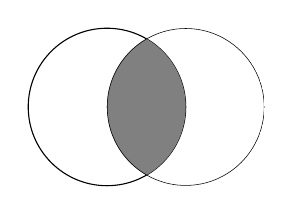
\begin{tikzpicture}
\begin{scope}
    \draw (1,0.7) circle (1cm);
    \clip (2,0.7) circle (1cm);
    \fill[gray] (1,0.7) circle (1cm);
    \draw (2,0.7) circle (1cm);
\end{scope}
\end{tikzpicture}
\end{center}
\item $\cup$, or the set \textbf{u}nion, is related to the logical or ($\lor$).

\item[] \begin{center} $\cup$NION \end{center}
\begin{center}
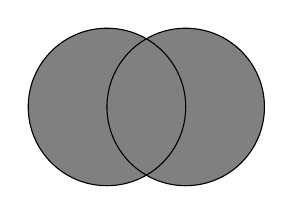
\begin{tikzpicture}
\begin{scope}
  
    \fill[gray] (1,0.7) circle (1cm);
        \fill[gray]  (2,0.7) circle (1cm);
          \draw (1,0.7) circle (1cm);
    \draw (2,0.7) circle (1cm);
 

\end{scope}
\end{tikzpicture}
\end{center}
\end{itemize}
\end{frame}




\begin{frame}
\frametitle{Set Rules}


\begin{itemize}
\item Commutative rules:
\begin{itemize}
\item $A \cup B = B\cup A$;
\item $A \cap B = B\cap A$;
\end{itemize}
\item Associative rules:
\begin{itemize}
\item $(A \cup B) \cup C = A \cup (B \cup C)$;
\item $(A \cap B) \cap C = A \cap (B \cap C)$;
\end{itemize}
\item Distributive rules:
\begin{itemize}
\item $A \cap (B \cup C) = (A \cap B) \cup (A \cap C)$;
\item $A \cup (B \cap C) = (A \cup B) \cap (A \cup C)$;
\end{itemize}
\end{itemize}
\end{frame}



\begin{frame}
\frametitle{Concise Notation for Set}

Oftentimes we don't want to (or can't) simply list all the items in a set, so we define sets in other ways (note  we \textit{always use the curly braces}) \pause

\begin{itemize}
\item The set of all the boys' names that start with a vowel: $\{x: x\hbox{ is a boy's name starting with a vowel}\}$
\item The set of all real numbers greater than -17.5 and less than 4: $\{x\in \mathbb{R}:-17.5<x<4\}$ \pause
\end{itemize}
 
Using this notation, we can define the following:
$$A\cup B=\{x: x\in A \hbox{ or } x\in B\}$$
$$A\cap B=\{x: x\in A \hbox{ and } x\in B\}$$

Note, $:$ means `such that'
\end{frame}



\begin{frame}
\frametitle{Set Theory}

Claim:  The empty set $\emptyset$ is a subset of every set. \pause

\ \\\underline{Direct proof}: First, note that $B\subset A$ is equivalent to the statement that $$\forall x\in B \hbox{ we have }  x\in A.$$ \pause

We want to prove that $\emptyset \subset A$ for any set $A$. \pause

This is equivalent to saying that for all $x\in \emptyset$, we have $ x\in A$.  But we know that $\not\exists x\in \emptyset$.  Therefore the statement that these (nonexistent) $x$ are in $A$ is vacuously true.  $\Box$

\end{frame}



\begin{frame}
\frametitle{Set Theory}

Other vacuously true statements: \pause

\underline{Claim}: If the moon was purple, then rain would fall up.

\underline{Definition}: A binary relation is \textit{quasitransitive} if $a>b$ and $b>c$ implies that $a>c$.

\underline{Claim}: The binary relation with $a=b$ and $b>c$ and $a=c$ is quasitransitive.

\end{frame}



\begin{frame}
\frametitle{Set Theory}

Claim:  The empty set $\emptyset$ is a subset of every set. \pause

\underline{Proof by contradiction}: First, note that $B\not\subset A$ is equivalent to the statement that $$\exists x\in B \hbox{ such that } x\not\in A. $$ \pause

Suppose that $\emptyset \not\subset A$.  \pause Then by the above statement we know that $\exists x\in \emptyset: x\not\in A$.  However, this contradicts the fact that $\not\exists x\in \emptyset$.  Thus, $\emptyset\subset A$.   $\Box$

\end{frame}


\begin{frame}
\frametitle{Family of Sets and Cardinality of Set}

\begin{itemize}
\item A \textit{family of sets} is a set whose elements are themselves sets
\begin{itemize}
\item $\{\{1, 2, 4\}, \{2, 6\}, \{\hbox{green}\}\}$ \pause
\end{itemize}
\end{itemize}

\begin{itemize}
\item A well-known family of sets is the \textit{power set} of any set $X$: it is the set of all subsets of $X$, and is written $2^X$ 
\begin{itemize}
\item How many ways can we create sets of $\{cat,\ dog\}$? \pause
\item $2^{\{\hbox{cat, dog}\}}=\{\emptyset, \{\hbox{cat}\}, \{\hbox{dog}\}, \{\hbox{cat, dog}\}\}$ \pause
\end{itemize}
\end{itemize}

\begin{itemize}
\item $|X|$ is the cardinality (size) of set $X$; the number of elements in $X$
\begin{itemize}
\item If $A = \{dog, cat\}$, $|A| =2 $\pause
\item If $|X|=n$ then $|2^X|=2^n$
\end{itemize}
\end{itemize}

\end{frame}



%\begin{frame}
%\frametitle{Conditional Statement}

%\begin{defn}
%"If P then Q" is sometimes called a conditional statement, with P as its antecedent and Q as its consequent. We can also write it as $P \rightarrow Q$.
%\end{defn} \pause

%\begin{itemize}
%\item Examples \pause
%\begin{itemize}
%\item If we are in the University of Chicago, then, we are in Chicago area. \pause
%\item If you get good grades, then, you will get into a good college. \pause
%\end{itemize}
%\end{itemize}

%\begin{itemize}
%\item Remark: If antecedent is not true, then the conditional statement is vacuously true.
%\end{itemize}

%\end{frame}



%\begin{frame}
%\frametitle{Conditional Statement: Truth Table}

%\begin{table}[]
%\begin{tabular}{llc}
%P & Q & \multicolumn{1}{l}{$P \rightarrow Q$} \\ \hline
%F & F & T?                                    \\
%F & T & ?                                     \\
%T & F & F                                     \\
%T & T & T                                    
%\end{tabular}
%\end{table}

%\end{frame}



%\begin{frame}
%\frametitle{And, Or}


%\begin{defn}
%Logical conjunction is an operation on two logical values, typically the values of two propositions, that produces a value of true if and only if both of its operands are true. It's denoted by $A \land B$.
%\end{defn}

%\begin{defn}
%Logical disjunction is an operation on two logical values, typically the values of two propositions, that has a value of false if and only if both of its operands are false. It's denoted by $A \lor B$.
%\end{defn}

%\end{frame}


%\begin{frame}
%\frametitle{Proof Strategies}

%Quick aside on proof strategies:

%\ \\Proof by contradiction: We want to show $A\Rightarrow B$.  Assume that both $A$ and $\neg B$ hold simultaneously.  Show that this implies a contradiction. \pause

%\ \\Proof by contrapositive: We want to show $A\Rightarrow B$.  Prove that $\neg B \Rightarrow \neg A$. \pause

%\ \\Proof by induction: We want to show that a property holds for all $n$, where $n$ is an integer.  (1) Prove it holds for $n=0$ (or $n=1$).  (2) \textit{Assume} it holds for arbitrary $n$.  (3) Prove it must hold for $n+1$.
%\end{frame}



%\begin{frame}
%\frametitle{Proof Strategies}

%Claim:  If $|X|=n$ then $|2^X|=2^n$ \pause

%\ \\\underline{Proof by induction}: Suppose that $|X|=0$.  If $X$ has no elements, then $X=\emptyset$. It follows that  $2^{\{\}}=\{\{\}\}$: the set of all subsets of $\emptyset$ is just the set containing $\emptyset$.  Thus, $|2^{\{\}}|=2^{|X|}=2^0=1$, proving our statement for $n=0$. \pause

%\ \\Suppose our statement holds for $|X|=n$, so $|2^X|=2^n$. \pause

%\ \\Let $Y=X\cup \{x\}$, so that $|Y|=n+1$.  $2^Y$ is $2^X\cup\{S: S\subset Y \text{ and } x\in S\}$.  Note that $2^X$ and $\{S: S\subset Y \text{ and } x\in S\}$ are disjoint. \pause

%\ \\The set $\{S: S\subset Y \text{ and } x\in S\}$ has $2^n$ elements: it is $\{S:  S=\{x\}\cup Z \text{ where } Z\in 2^X\}$.  Thus, $|2^Y| = 2^n+2^n=2*2^n=2^{n+1}$. This proves our result. $\Box$
%\end{frame}



\begin{frame}
\frametitle{Complementary Set Properties}

\begin{itemize}
\item If $A\subset B$ then the set of things that are in $B$ but not $A$ is the \textit{complement of $A$ in $B$} \pause

$$B\setminus A= \hbox{ The complement of $A$ in $B$} = \{x\in B: x\not\in A\}= B\cap A^c$$ \pause

\item Formally we often define complements with respect to an unstated universal domain:
$$A^c=U\setminus A$$
or 
$$A^c=\{x\in U|x\notin A\}$$
\item De Morgan's laws:
\begin{itemize}
\item $(A\cup B)^c=A^c\cap B^c$.
\item $(A\cap B)^c=A^c\cup B^c$.
\end{itemize}

\end{itemize}
\end{frame}


\begin{frame}
\frametitle{Using Definition of Complement}

\begin{itemize}
\item Prove that $(A^c)^c=A$\pause
\item[1)] Definition of $^c$ is that $x \in A^c \iff x\notin A$\pause is equivalent to the statement:
\item[] $x \notin A^c \iff x\in A$.\pause
\item[2)] So $x \in (A^c)^c \iff x\notin  A^c$ \pause
\item $x \notin A^c \iff x\in A$

\end{itemize}
\end{frame}


\begin{frame}
\frametitle{Important Sets of Numbers}

\begin{itemize}
\item A \textbf{finite} set contains a finite number of elements. \pause

\item An \textbf{infinite} set contains an infinite number of elements.

\item The set of real numbers, $\mathbb{R}$: All numbers that are positive, negative, or 0 \pause

\item The set of natural numbers, $\mathbb{N}$: The set of all strictly positive integers \\$\mathbb{N}=\{1, 2, 3, 4, ...\}$ \pause

\item The set of integers, $\mathbb{Z}: $ the natural numbers, their negatives, and 0\\$\mathbb{Z}=\{..., -2, -1, 0, 1, 2 ...\}$
\end{itemize}

\end{frame}



\begin{frame}

END VIDEO

\end{frame}


\begin{frame}

\begin{itemize}
\item \textcolor{mygray}{Course context}
\item \textcolor{mygray}{Set Theory}
\item \textcolor{myblack}{Vectors and Ordered Lists}
\item \textcolor{mygray}{Functions}
\end{itemize}

\end{frame}



\begin{frame}
\frametitle{Why Vectors and Ordered Lists}
\begin{itemize}
\item Sets ignore order, but we often have a collection of data where each value corresponds to a feature.\pause
\item For example, my pet has (at least) three attributes: a species (dog) a gender (female) and a name (Maeby).\pause
\item The set \{dog, female, Maeby\} would lose this ordering.\pause
\item The vector and ordered list saves these placeholder data.\pause
\item In our work, we will see most data is in the form of either a vector (if it is pure numbers) or an ordered list (if it is a mix of kinds of data).
\end{itemize}
\end{frame}


\begin{frame}
\frametitle{Ordered List}

\begin{itemize}
\item  Unlike sets, \textit{ordered lists} are denoted with smooth brackets $(c, a, b, d, e)$ \pause
\begin{itemize}
\item Elements can repeat \pause
\item These are sometimes called sequences.
\end{itemize}
\item The 2-dimensional plane is represented by $\mathbb{R}^2$, or $\mathbb{R}\times \mathbb{R}$

$$\mathbb{R}^2=\{(x, y): x\in \mathbb{R} \hbox{ and }y\in \mathbb{R} \}$$
\item The 3-dimensional space is represented by $\mathbb{R}^3$:

$$\mathbb{R}^3=\{(x, y, z): x\in \mathbb{R} \hbox{ and }y\in \mathbb{R}\hbox{ and } z\in \mathbb{R}  \}$$
\end{itemize}

\end{frame}



\begin{frame}
\frametitle{Cartesian Product}

\begin{itemize}
\item Ordered pairs can be generalized to any two objects, the possibilities are given by the Cartesian Product.

\item Given two sets $X$ and $Y$, the Cartesian product of $X$ and $Y$ is $\{(x, y): x\in X \hbox{ and }y\in Y\}$

\begin{itemize}
\item $\{\hbox{cat, dog}\}\times \{a, b\}= \{(\hbox{cat}, a), (\hbox{cat}, b), (\hbox{dog}, a), (\hbox{dog}, b)\}$ \pause
\item $X_1\times X_2\times ... \times X_n=\{(x_1, x_2, ..., x_n):x_i\in X_i \hbox{ for }i=1, 2, ..., n\}$ \pause
\end{itemize}
\end{itemize}

\begin{itemize}
\item $\mathbb{R}^n$ is the $n$-ary Cartesian product of $\mathbb{R}$
$$\mathbb{R}^n=\{(x_1, x_2, ..., x_n): x_i\in \mathbb{R} \}$$
\item $\mathbb{R}^2$ is the typical 2d plane
\item $\mathbb{R}^3$ is the 3d space
\end{itemize}

\end{frame}







\begin{frame}
\frametitle{Vector}

\begin{defn}
An ordered list of numbers is a \textit{vector}.
\end{defn}
\pause

If the vector has $n$ elements, then it is an element of $n$-dimensional Euclidean space, or $\mathbb{R}^n$ \pause

{Examples: }
\begin{itemize}
\item $(1, 5, 7)\in \mathbb{R}^3$
\item $(3, 2, 7, 12, 65, 78787, 3)\in \mathbb{R}^7$ \pause
\end{itemize}

{Remark: }
\begin{itemize}
\item If $n\leq 3$, you can plot out the vector (as either on a line, the plane, or 3-D space).
\item In R, we write a vector with c():
\item[] \texttt{c( 25, 30, 40)}
\end{itemize}

\end{frame}

\begin{frame}{Analogy from data to coordinates}

\begin{itemize}
\item It is useful to be able to think about vectors either as an ordered list of numbers or as a point in space. 
\item The analogy to space offers insights, but is limited to vectors of length less than 3.
\item The data encoded in a length 2 vector $(a, b)$ can be used to describe an arrow from the origin to the point $x = a$, $y =b$
\end{itemize}

\end{frame}


\begin{frame}{Outline}

\begin{itemize}
\item \textcolor{mygray}{Course context}
\item \textcolor{mygray}{Set Theory}
\item \textcolor{mygray}{Vectors and Ordered Lists}
\item \textcolor{myblack}{Functions}
\end{itemize}

\end{frame}


\begin{frame}
\frametitle{Why Functions?}
\begin{itemize}
\item Functions describe regularity: the fundamental target of science.
\item Theoretical work relies on functions to describe relationships.
\item Random variables are functions (more on that later).
\item Here we just introduce some basic terminology.
\end{itemize}
\end{frame}



\begin{frame}
\frametitle{Mathematical Functions}
\begin{defn}
A \textit{function} is a mapping from a set $X$ into a set $Y$
\end{defn}
\pause

\begin{itemize}
\item This means that for each element of $X$, $f$ assigns an element of $Y$, or $f: X\rightarrow Y$ \pause
\end{itemize}

\begin{itemize}
\item The \textit{graph} of a function from $\mathbb{R} $ to $\mathbb{R}$ is the set $$\{(x, y)\in \mathbb{R}^2: y=f(x)\}$$ 
\end{itemize}
\end{frame}



\begin{frame}
\frametitle{Aside on variables}
\begin{defn}
The letters $X$, $Y$, $A$, $B$, $x$, $y$ are \emph{variables}.
\end{defn}
\pause

\begin{itemize}
\item Common to use script upper and lower case letters.
\item We will also use the Greek letters.

\item[] alpha $\alpha$ ; beta $\beta$ ; gamma ; $\gamma\Gamma$ ; delta $\delta\Delta$ ; epsilon $\epsilon$ ; zeta $\zeta$ ; eta $\eta$ ; theta $\theta\Theta$ ; iota $\iota$ ;  lambda $\lambda\Lambda$ ; mu $\mu$ ; nu $\nu$ ; omicron o ; pi $\pi\Pi$ ; \\
 rho $\rho$ ; sigma $\sigma\Sigma$ ; tau $\tau$ ; upsilon $\upsilon\Upsilon$ ; phi $\phi\Phi$ ; chi $\chi$  ;\\
 psi $\psi\Psi$ ; omega $\omega\Omega$
\item As a last resort, we go to the Hebrew ($\aleph \beth \daleth \gimel$)
\end{itemize}


\end{frame}



\begin{frame}
\frametitle{Classes of Functions}

\begin{defn}
A function $f: X\rightarrow Y$ is \textit{one-to-one} (or injective) if every element of $X$ maps into a unique element of $Y$ ($f(a)=f(b)\Rightarrow a=b$)
\end{defn}
\pause

\begin{defn}
A function $f: X\rightarrow Y$ is \textit{onto} (or surjective) if every element of $Y$ is mapped into by some element of $X$ ($\forall y\in Y, \exists x\in X: f(x)=y$) \pause
\end{defn}

\begin{defn}
A function that is \emph{one-to-one} and \emph{onto} is \emph{bijective}
\end{defn}

\end{frame}

\begin{frame}{Aside on logic terms}

\begin{itemize}
\item For all $\forall$, exists $\exists$, if and only if $\iff$
\begin{itemize}

\item $\forall y\in Y, \exists x\in X: f(x)=y$ : ``For all $y$ in the set $Y$, there exists an $x$ in the set $X$ such that the function f evaluated at $x$ is equal to $y$.

\item $\nexists a \in Y \iff \forall y \in Y,  y\neq a$ : There does not exist an element $a$ in the set $Y$ if and only if for all elements $y$ in the set $Y$, $y$ is not equal to $a$.
\end{itemize}
\end{itemize}
\end{frame}



\begin{frame}
\frametitle{Test Your Understanding}

\begin{itemize}
\item $f: \mathbf{R}\rightarrow \mathbf{R}$ $f(x)=x^2$ is injective and surjective
\item $g: \mathbf{R}\rightarrow \mathbf{R}$ $f(x)=x^3$ is surjective
\item  $g: \mathbf{R}\rightarrow \mathbf{R}$ $f(x)=x^3-3x$ is injective
\end{itemize}
   
\end{frame}

\begin{frame}
\frametitle{Test Your Understanding}


\begin{itemize}
\item $f: \mathbf{R}\rightarrow \mathbf{R}$ $f(x)=x^2$ is injective and surjective FALSE, neither is true.
\item $g: \mathbf{R}\rightarrow \mathbf{R}$ $f(x)=x^3$ is surjective TRUE. 
\item  $g: \mathbf{R}\rightarrow \mathbf{R}$ $f(x)=x^3-3x$ is injective FALSE, it is surjective.
\end{itemize}
   
\end{frame}

\begin{frame}
\frametitle{Composite Functions}
Functions can be combined.  When they are, they are called composite functions:
\begin{defn}
 If $f:B\rightarrow C$ and $g: A\rightarrow B$ then \\$f\circ g = f(g(x))$ is a mapping from $A$ to $C$: $x\in A$, $g(x)\in B$, and $f(g(x))\in C$
\end{defn}

\end{frame}


\begin{frame}{Composite Function Example}

\begin{itemize}
\item $f: \mathbb{R}^2\rightarrow \mathbb{R}$, with $f(x, y)=x+2y$ 

\item $g: \mathbb{R}^3\rightarrow \mathbb{R}^2$, with $g(x, y, z)=(x^2+2y*z, 7)$ \pause
\end{itemize}

\begin{itemize}
\item $$h(x,y,z)=f\circ g=f(g(x,y,z),y): \mathbb{R}^3\rightarrow\mathbb{R}, \text{ with }$$
$$h(x, y, z)=x^2+2y*z+14$$\pause

\end{itemize}

\end{frame}


\begin{frame}
\frametitle{In-class problems}

\begin{itemize}

\item[3.1.2] Let $A, B, C$ be sets such that $A\subset B$ and $A\cap C=\emptyset$.  Simplify the following, if possible:

\begin{itemize}
\item $A\cap(B\cup C)$ %A
\item $(A\cap B)\cup C$ % A\cup C
\item $A\cup(B\cap C)$ %No simplification 
\item $(A\cup B)\cap C$ %B\cap C


\end{itemize}

\end{itemize}
\end{frame}


\begin{frame}
\frametitle{In-class problems}

\begin{itemize}
\item Let $f:\mathbb{R}^2\rightarrow \mathbb{R}^2$. Interpret the mapping $f(x, y)=(x, -y)$ geometrically
\begin{itemize}

\item Which points remain unchanged under this mapping? %It's the reflection about the x-axis.  The x-axis is unchanged.

\item Now answer both questions for $f(x, y)=(x, -4)$ % Projection onto line y=-1. Unchanged points are along the line y=-4.

\end{itemize}
\end{itemize}

\end{frame}

\begin{frame}{Important things from Pemberton and Rau}

\begin{itemize}

\item How to sketch functions.
\item Linear programming.
\item Real, rational, irrational numbers.
\item \textcolor{myblack}{Functions}
\end{itemize}

\end{frame}

\end{document}
